\documentclass{acm_proc_article-sp}

\begin{document}

\title{DataSeries: an efficient, flexible data format for structured serial data}
% Pretend we have one author, minimizes the space we waste on that.
\numberofauthors{1} 
\author{
\alignauthor
Eric Anderson, Martin Arlitt, Brad Morrey, Alistair Veitch  \\
 \affaddr{HP Labs. 1501 Page Mill Rd.  Palo Alto, CA} \\
 \email{\{eric.anderson4, martin.arlitt, brad.morrey, alistair.veitch\}@hp.com}
}

\maketitle
\begin{abstract}

DataSeries is an on-disk data format, run-time library, and set of
tools that is optimized for analyzing \textit{structured serial data},
which we define as an ordered series of records that share a common
structure.  This type of data commonly occurs as trace data in
computer systems, but since the format is essentially ordered RDBMS
tables, the need to maintain and analyze such data occurs in a large
number of scientific fields.

DataSeries has been optimized to be extremely space and CPU efficient,
while providing the flexibility to accommodate a very wide range of
record structures. We demonstrate the flexibility by describing the
many different types of data we have stored and analyzed in
DataSeries.  We examine the efficiency of DataSeries on a subset of
these types and demonstrate three improvements: 1) processing rates up
to two orders of magnitude better than existing formats; 2) ability to
store and analyze traces with hundreds of billions of records on
low-end servers; 3) compression ratios somewhat better than existing,
specialized formats when using the same generic compression algorithm,
and much better when compared to formats without built-in
compression. 

Finally, DataSeries software is open source, enabling others to take
advantage of these benefits.

\end{abstract}

% % A category with the (minimum) three required fields
% \category{H.4}{Information Systems Applications}{Miscellaneous}
% %A category including the fourth, optional field follows...
% \category{D.2.8}{Software Engineering}{Metrics}[complexity measures, performance measures]
 
% \terms{Structured serial data}

% \keywords{ACM proceedings, \LaTeX, text tagging} % NOT required for Proceedings

\section{Introduction}

Traces, recordings and measurements taken from computer systems,
networks and scientific infrastructure are vitally important for a
large variety of tasks. In every area of computer system design,
traces from existing systems have been used to validate hypotheses,
test assumptions and estimate performance. This is true of I/O
subsystems~\cite{IORef,Ji03,Uysal03}, processor
systems~\cite{ProcRef}, network systems~\cite{NetRef} and memory
systems~\cite{MemRef}, among others. Traces and logs are also
extremely useful for fault-finding, auditing and debugging purposes
~\cite{DebugRef}. Traces composed of failure data have been used to
determine system reliability~\cite{ReliabilityRef, Schroeder07,
Pinheiro07}. Trend analyses of performance information is a core
operation of various management tools~\cite{MgmtRef}. Specific to the
area of I/O and storage systems alone, we found that almost 60\% of
papers published in the File and Storage Technologies (FAST)
conferences have used traces of one sort or another.  Scientific and
medical instrumentation can also generate large amounts of
data~\cite{SciRef}, which also needs to be stored, filtered and
analyzed.

The data stored in each of these diverse uses is {\it structured
serial data}, which we define as a series of records, each record
having a specified structure (i.e., containing the same set of
variables). Structured serial data has four defining characteristics:
its structure is record-oriented; it is typically written only once,
not modified afterward, and is read many times; it is usually ordered
in some manner, e.g., chronologically; and it is typically read in a
sequential manner.  Traditionally, researchers and developers have
accomplished the tasks of collecting, storing, and analyzing this type
of data using formats, libraries and software which are customized to
the particular task at hand.  Unfortunately, such approaches
significantly limit both flexibility and reusability, and often
performance.  For instance, if a binary format is used, it may be
difficult to add new items of information or remove obsolete
information.  More flexible formats (e.g., text or XML) are not
amenable to efficient analysis or storage.  Traditional databases
generally store data without compression, requiring large amounts of
disk space for storage, and are typically not optimized for the
specific types of processing used on structured serial data.  One of
the key contributions of this work is the specific storage format and
optimizations that make it possible to very efficiently store and
analyze this type of data, without requiring excessive amounts of disk
storage or computational resources.

Another, often overlooked advantage of having a one-size-fits-all
trace format is the ease of use provided in data analysis. In our own
work, we have combined disparate trace types (block level I/O, process
accounting, system call, NFS, batch scheduler, and system performance
traces) in various combinations. Having a single software system and
trace format that can work with each of these trace types through
merge and analysis operations greatly facilitates the ease of
analysis. A related advantage is scientific; reproducibility is
enhanced and interpretation is simplified.  The authors have
experienced, both personally and anecdotally, the difficulty of
reproducing results with ``old'' trace files and software (often just
finding software and getting it to compile can be extremely
problematic). We observe that of the 101 papers published in the
history of FAST, 57 used traces in some way; the traces used in these
papers were of at least 45 different formats.  Several papers even
used 4-5 different types (e.g.,~\cite{arc03, ellard03}).

There are five key properties that are desired of a data format
and analysis system for structured serial data:

\begin{enumerate}

\item \textbf{Storage efficiency}: the data should be stored in as few
bytes as possible.

\item \textbf{Access efficiency}: accessing, interpreting and encoding
trace data, whether reading or writing, should make efficient use of
CPU and memory resources.

\item \textbf{Flexibility}: adding additional fields should not affect
users of the trace data.  Removing or modifying data fields should
only affect users who use those fields and the system should support
catching incorrect usage.  Further, the format should not constrain
the type of data being stored, and should allow multiple record types
in a single file.

\item \textbf{Self-describing}: the data set should contain the
metadata that describes the data.

\item \textbf{(Re)Usability}: the data format should have an associated
programming interface that is both expressive and easy to use.

\end{enumerate}

Although numerous tracing and measurement systems have been developed
over the last 20-30 years, we are not aware of any that meet all of
these requirements. We analyze some of these in our description of
related work (section~\ref{sec:related}).

We provide four primary contributions in this paper.  First, we
introduce DataSeries, a data format and associated library, which was
specifically designed to meet the five key properties discussed above.
Second, we discuss how DataSeries can support very large datasets
(e.g., hundreds of billions of records) on modest systems.  Third, we
describe how we have used DataSeries in practice to store a wide
variety of data types.  Fourth, we demonstrate the performance and
storage efficiency of DataSeries in a set of controlled experiments,
using empirical data sets. We show that the performance of DataSeries
exceeds the performance of common trace formats and databases by at
least a factor of two, and in some cases up to an order of
magnitude. DataSeries also requires far less disk space (factors vary
from 4X to 8X in test workloads).

Since DataSeries software is publicly available (under a BSD software
license), and given the benefits of DataSeries that we demonstrate, we
argue that DataSeries should be considered for use by any application
that needs to store large amounts of structured serial data. Indeed, a
storage industry group\footnote{name withheld for blinding purposes}
has chosen DataSeries as a standard format for I/O trace data, and is
currently specifying the semantics of the fields.

The remainder of this paper is organized as follows.
Section~\ref{sec:related} describes the strengths and weaknesses of
existing storage technologies relative to DataSeries.
Section~\ref{sec:design} describes the design of DataSeries, including
on-disk and in-memory formats.  Section~\ref{sec:programming}
describes the programming interface for DataSeries.
Section~\ref{sec:results} presents empirical and benchmark results
from our use of DataSeries to illustrate and quantify the benefits of
DataSeries.  Section~\ref{sec:discussion} describes our experiences
with using DataSeries, and Section~\ref{sec:conclusions} concludes the
paper with a summary of our work and a list of future directions.

\section{Related Work}\label{sec:related}

We classify the related work into three categories:
those that use a customized binary format, those that use a
text-based format, and relational database systems. 

Custom binary formats are usually serialized or directly written
versions of an in-memory data structure.  As such, they usually
achieve properties 1 and 2, and fail to achieve properties 3-5,
although as we will show in the results, unless the authors are
careful, they can also fail to achieve property 2.

Text base formats such as column separated value, or XML usually
achieve properties 3 and 4, and XML achieves property 5.  However,
they fail to achieve property 1, and can fail property two by multiple
orders of magnitude.  As we show in our results even very tuned CSV
implementations can only get to within 2-7$\times$ the
access-efficiency of DataSeries, and x-y$\times$ for the storage
efficiency.  {\bf TODO: need to re-do these experiments at least to
measure the file sizes, and potentially with Tfrac text files,
although I suspect people would use sec.usec in a block I/O trace}

Relational databases achieve properties 3, 4, and 5. RDBMS's were
designed to handle updates, so do very limited compression drastically
hurting their storage efficiency (property 1).  Our results show
$>$10x improvement on storage efficiency for DataSeries over
MySQL. {\bf TODO: check the exact sizes, should be around there.}
Similarly, the generality of SQL can hurt it.  Even for fairly simple
queries running entirely in the database, DataSeries runs 2-7$\times$
faster than MySQL. {\bf TODO: re-do these numbers with parallel
decompression, etc.}  Retrieving the data for a more complicated
calculation on the client would further slow the relative performance.

\section{Design}\label{sec:design}

\begin{figure*}
% \vspace{-0.6cm}
\hfil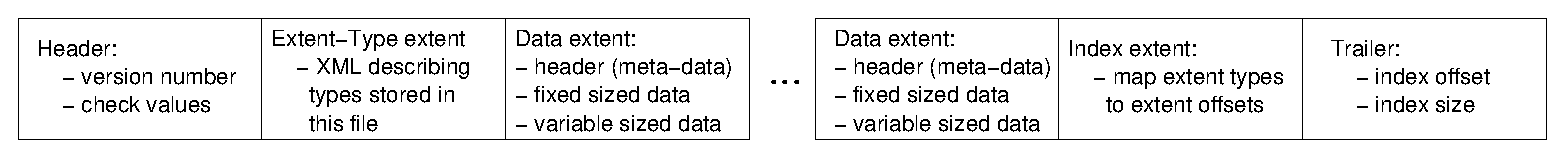
\includegraphics[width=6.5in]{tr-fig/ds-format2.eps}\hfil
\caption{Internal structure of a DataSeries file. }
\label{fig:dsorg}
% \vspace{-2mm}
\end{figure*}

\section{Programming}\label{sec:programming}

...

\section{Performance Results}\label{sec:results}

...

\begin{table}
\centering
\begin{tabular}{|c|c|c|c|}\hline

               &            & ratio to & ratio to \\
    dataset    & size (MiB) & ds-base & be-bts-gz \\
\hline							   
ds-mcs-bts-tsr & 7648.98  & 1.133         & 1.077         \\
be-bts-gz      & 8239.15  & 1.052         & 1.000         \\
ds-base        & 8663.78  & 1.000         & 0.951         \\
\hline
\hline
\end{tabular}

\caption{Compression options for the data files sorted from the smallest 
to the largest.  Gzipped files can be stored little or big endian
(le/be) and small to big or big to small (stb/bts).  DataSeries files
can be stored with the fields padded only to the maximum column size
(mcs), with the fields stored big to small (bts), or with the time
field packed self relative (tsr). be-bts-gz is the original 1998 World
Cup trace format.}

\label{table:wc1998:compression}
\end{table}

\section{Discussion}\label{sec:discussion}

...

\section{Conclusions}\label{sec:conclusions}

...

DataSeries is open source that can be downloaded from {\tt
http://tesla.hpl.hp.com/opensource/}

\bibliographystyle{abbrv}
{\small
\bibliography{tr-references}
}
% You must have a proper ".bib" file
%  and remember to run:
% latex bibtex latex latex
% to resolve all references
%
% ACM needs 'a single self-contained file'!
%
\balancecolumns

\end{document}
